% --------------------------------------------------------------
% This is all preamble stuff that you don't have to worry about.
% Head down to where it says "Start here" % --------------------------------------------------------------
 
\documentclass[12pt]{article}

\usepackage{listings}
\usepackage[margin=1in]{geometry} 
\usepackage{amsmath,amsthm,amssymb}
\usepackage{graphicx}
\usepackage{hyperref}
\graphicspath{ {../} } 

\newcommand{\N}{\mathbb{N}}
\newcommand{\Z}{\mathbb{Z}}
\newcommand\indep{\protect\mathpalette{\protect\independenT}{\perp}}
\def\independenT#1#2{\mathrel{\rlap{$#1#2$}\mkern2mu{#1#2}}}

\newenvironment{theorem}[2][Theorem]{\begin{trivlist}
\item[\hskip \labelsep {\bfseries #1}\hskip \labelsep {\bfseries #2.}]}{\end{trivlist}}
\newenvironment{lemma}[2][Lemma]{\begin{trivlist}
\item[\hskip \labelsep {\bfseries #1}\hskip \labelsep {\bfseries #2.}]}{\end{trivlist}}
\newenvironment{exercise}[2][Exercise]{\begin{trivlist}
\item[\hskip \labelsep {\bfseries #1}\hskip \labelsep {\bfseries #2.}]}{\end{trivlist}}
\newenvironment{reflection}[2][Reflection]{\begin{trivlist}
\item[\hskip \labelsep {\bfseries #1}\hskip \labelsep {\bfseries #2.}]}{\end{trivlist}}
\newenvironment{proposition}[2][Proposition]{\begin{trivlist}
\item[\hskip \labelsep {\bfseries #1}\hskip \labelsep {\bfseries #2.}]}{\end{trivlist}}
\newenvironment{corollary}[2][Corollary]{\begin{trivlist}
\item[\hskip \labelsep {\bfseries #1}\hskip \labelsep {\bfseries #2.}]}{\end{trivlist}}
 
\begin{document}
 
% --------------------------------------------------------------
%                         Start here
% --------------------------------------------------------------
 
%\renewcommand{\qedsymbol}{\filledbox}
 
\title{Assignment 2\\
Big Data Analytics Programming} %if necessary, replace with your course title
\author{Evangelos Ntavelis\\ %replace with your name
r0692337 \\
evangelos.ntavelis@student.kuleuven.be}
 
\maketitle

\tableofcontents

\section{Introduction}
Firstly, we are are going to discuss the choices that were made when implementing the LSH algorithm. Afterwards we are discuss the effect of the parameters' values on the task performance and execution time and lastly we are going to motive our choice for parameter for running on the whole dataset.

\section{Implementation Choices}

There are two major keywords describing our approach to developing the solution for this assignment: Objects and Hash-Maps/Sets.

In order to be able to write code in a sustainable and manageable manner we followed the objected oriented principle.
We had both LSH and BruteForce classes to extend a basic Searcher Class.
We also created a class for the Universal Hash to help us structure better the creation of the Signature Matrix. This later proved useful as we also Implemented a second LSH class for short Signatures.

A very important choice during the implementations was the data structures we used. For the most of the  cases a HashSet provided the most performant solution.
Yet, for the case of the Signature Matrix a two dimensional array provided a better solution due to the dense nature of the Data. 

There were three ways to implement the \textbf{Universal Hash}: store the hash values on an array or a HashSet or call the function each time. By testing all approaches we found out that even for large shingles, the array solution is the best (3 quicker than HashSet and better than function calling). However, when dealing with the whole dataset we found out that for small shingle numbers it was better to store an array but for bigger to just call the function. Having two implementations for short and integers permitted us to implement this both ways according to the shingle size. 

The design and creation of the \textbf{Signature Matrix} was the most important aspect of our program both time-wise and space-wise. The first important choice was in cases we are using a number of shingles that can fit into \textit{Short Type} and by doing so we could half the space needed and improve the overall time. We created two version of LSH, one with short signatures and one for Integers.

Given also the way java saves multi-dimensional arrays in memory it made sense to create $\#MinHashes \times Arrays-of-\#Tweets$ both because the number of tweets is a lot bigger than the MinHashes as well ass the way we traverse the Matrix at its creation and the buckets assignment. This way we have less Cache Misses.

Another significant choice was how to handle the \textbf{Similarity Pairs}. We wanted to make sure that there are no duplicates in our Similar Pairs HashSet but also we didn't want to check the similarity of pairs we have already decided they are similar. In order to do, so we added the functions \textit{equals()} and \textit{hashCode()} to the Similarity Class. We followed the language guidelines to make sure that the two functions are designed as intended \footnote{http://programmergate.com/working-hashcode-equals-java/}. If two Pairs end up being in the same bucket we first check if we have already assigned as similar and we don't redo the calculations. However, if the two pairs have already been checked for similarity and got rejected, if they hash in to the same bucket again for another band, we are going to redo the calculations. The reason is that the probability of finding again a rejected pair is quite low if we take into account that a subset of the signatures which are similar was not enough to deem them similar, and thus we didn't want to introduce an overhead to check this out. The effect is larger when the threshold is smaller. Also, we made sure that the Pairs are examined by having the smaller id always first.

In order to measure and evaluate the solutions we used Python. We run the experiments locally and we used Python to calculate the TN, FP, FN as well as the derived performance metrics: Precision, Recall and F1-score and execution time.

A last remark: we  could also try to write parallel code both for the transformation to the Signature Matrix, document-wise as well to the bucket assignment procedure, band-wise.


\section{Parameter Analysis}


\textbf{Number of Shingles:} As the size of the vocabulary grows larger we expect to have more collisions in the Shingle Hashing process if we don't accordingly increase the number of Shingles. 

More collisions mean that that our algorithms, both BruteForce and LSH, we'll predict more False Positives as it will regard different substrings as same. On the other hand there is a point where increasing the number of shingles won't alter the result. There if we don't have a significant difference in performance due to the HashSet implementation, by using a Number of Shingles that can be represented by a \textit{Short Type} we can save half the space we are using. This in fact permits us to double the size our \textit{Signature Matrix} before reaching our limits when dealing with \textit{Big Data}.

Moreover, we found out that for the 100.000 sample the while we have a significant improvement in precision from 1000 to 10.000 shingles ($0.8 \rightarrow 0.875$ for 8 bands and 10 rows), it flats out when going to 100.000 and 1.000.000 shingles.  

Our insight agrees to the empirical results for 100.000 tweets on the following table.

\begin{center}
 \begin{tabular}{||c |  c||}
 \hline
 Nb of Shingles & BruteForce Pairs  \\ [0.5ex]
 \hline\hline
 1000 & 7232  \\
 \hline
 10000 & 6955  \\
 \hline
 100000 & 6955 \\
 \hline
\end{tabular}
\end{center}

\textbf{Shingle Length:} By increasing the shingle length we observed the execution time going up, while recall value was going down and precision going up. The increase in time is expected as the reading takes k*all characters steps. Increasing the K will result to more combinations and to reduce the collisions we should also increase the number of shingles.

\textbf{Threshold:} By using the same combination of bands and rows as for the 0.9 threshold, we can see the effect described in the pdf and shown in Figure 5. The high S-curve threshold makes our model to produce nearly no False Positives but it Produces a lot of FN as well (2 times the TN). As expected, we are dealing with a lot more predictions both on the lsh and the brute force algorithm. Yet we can manipulate the performance in a similar way with higher thresholds using the S-curve theory.

\begin{center}
 \begin{tabular}{||c |  c||}
 \hline
 Threshold & \#Pairs \\ [0.5ex]
 \hline\hline
0.5 & 35162 \\
 \hline
0.7 & 18383 \\
 \hline
0.9 & 6955 \\
 \hline
\end{tabular}
\end{center}

\textbf{Number of Buckets:} Having a small number of buckets compared to the number of tweets we examine has a bad effect on both regards. Pigeonhole principle states that having less ``holes/buckets'' than ``pigeons/tweets'' will result to collisions. The more collisions we have the more dissimilar pairs we are going to check. The number of similarity checks grows exponentially as the number of the tweets per document increase. Here we don't have a problem to increase the number of buckets as it doesn't affect the execution time as we see in the following table which describes the running time for 10 runs and 100.000 tweets locally: 

\begin{center}
 \begin{tabular}{||c |  c||}
 \hline
 Nb of Buckets & 10*Execution Time(sec) \\ [0.5ex]
 \hline\hline
1000 & 786 \\
 \hline
10000 & 184 \\
 \hline
100000 & 122 \\
 \hline
1000000 & 113 \\
 \hline
10000000 & 109 \\
 \hline
\end{tabular}
\end{center}

We can observe that the time goes down exponentially. At the same time we don't have any differences performance-wise.

\begin{figure}[t]
\caption{Precision}
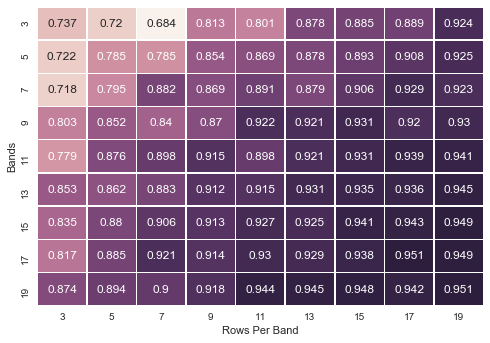
\includegraphics[scale=0.7]{precision.png}
\centering
\end{figure}


\begin{figure}[t]
\caption{Recall}
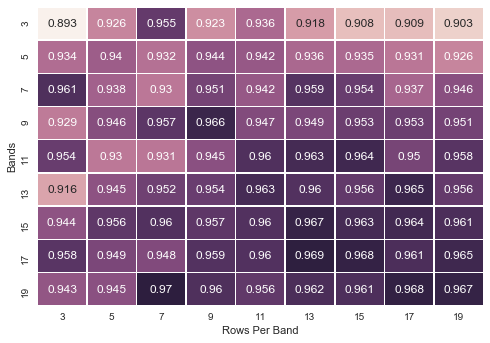
\includegraphics[scale=0.7]{recall.png}
\centering
\end{figure}


\begin{figure}[t]
\caption{F1-score}
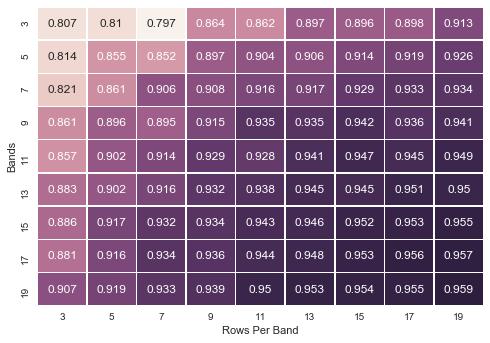
\includegraphics[scale=0.7]{fscore.png}
\centering
\end{figure}


\begin{figure}[t]
\caption{Execution time}
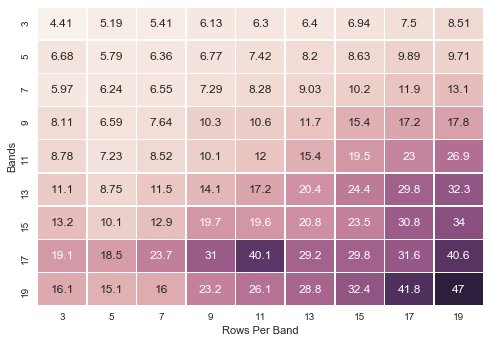
\includegraphics[scale=0.7]{time.png}
\centering
\end{figure}


\textbf{Signatures, Bands and Rows per Band}. These three parameters are the most important and can be regarded as two as:
\[ Bands * RowsPerBand = \#Signatures\]

The experiments of the results presented here were run with the following settings, and the results is the average of 5 running times:

For all cases we can see that 
\begin{center}
 \begin{tabular}{||c |  c||}
 \hline
 Parameter & Value \\ [0.5ex]
 \hline\hline
nTweets & 100.000 \\
 \hline
nShingles & 10.000 \\
 \hline
ShingleLenght & 3 \\
 \hline
nBuckets & 100.000  \\
 \hline
Threshold & 0,9 \\
 \hline
\end{tabular}
\end{center}

We can observe the following:

\begin{itemize}
    \item As we increase the signature size (moving down- and left-wards) we are increasing the overall performance but the execution time also increases. 
The size of the signature matrix was the biggest bottleneck on the execution time.   
    \item By keeping the number of signatures(minHashes) constant we find out that as we increase the number of rows and decrease the number of bands we increase the precision but decrease the recall value. The f1-score remains approximately the same. Yet as precision goes up, both FPs and TPs go down. 
    \item Especially when running on the whole dataset we can observe the differences in execution time:   
    
  \end{itemize}

\begin{center}
 \begin{tabular}{||c  | c |  c||}
 \hline
 Bands & Rows & Running Time \\ [0.5ex]
 \hline\hline
 20  & 4 &  1:03:47 \\
 \hline
 4 & 20 &  0:07:36\\
 \hline
\end{tabular}
\end{center}


\textbf{Short VS Integer Signatures} There were many experiments that took place in order to evaluate which way is the better. We found that by setting the number of Shingles to 1 million, we produce 
$152643$ distinct shingles for the our 100.000 sample and $415500$ for the whole dataset. Following the chart of characters 3-grams for \textit{Zipf's law}\footnote{I. Sicilia-Garcia, E \& Ming, Ji \& J. Smith, F. (2009). Extension of Zipf’s Law to Word and Character N-Grams for English and Chinese. 8. . } we expect the additional shingles to be less frequent that those observed firstly in our sample. We also found that maximumly at 10.000 shingles the performance evens out for our sample set. Based on the above we can argue that $~32.000$ Shingles will be enough, given the execution time and storage boost.


\section{Going Big (Data)}

There are two things we want to optimize: execution time and TP/FP performance. The first is pretty straight forward, for the latter we will try to maximize the value of precision as:
\[precision = \frac{TP}{TP + FP}\]


\begin{itemize}
    \item
    We picked the Shingles Number to be equal to the MaxValue a Short Number can take. This permitted us to increase the Signature Size
    \item 
      We picked the buckets to be 10.000.000 following the experiments we made on the sample dataset: Less collision without overhead.
    \item 
      In order to maximize the precision and also minimize the running time we will pick $Rows >> Bands$.  
    \item
    We also choose the configuration based on the chapter provided on the assignment and following the lovely table on Figure 5 where the values of $(1/b)^{1/r}$ are computed. We pick a threshold bigger than 0.9 as we wanted to produce less FP and have less execution time.
    \item One thing that we encountered during experimenting on the departmental machines, sometimes some configurations work and others don't. We attribute this to the different load that certain machines are facing at certain times. It was made sure that the solution can be run in different machines and at different times with different workloads.

      \item Finally, we picked 4*20 instead of 4*25, because of the execution time gain and the less memory needed.


\end{itemize}

\begin{center}
 \begin{tabular}{||c |  c||}
 \hline
 Parameter & Value \\ [0.5ex]
 \hline\hline
Bands & 4 \\
 \hline
RowsPerBands & 20\\
 \hline
nShingles & 32.000 \\
 \hline
nBuckets & 10.000.000  \\
 \hline
 \hline
Running Time & real 06:14m (@Namen) \\

 \hline

\end{tabular}
\end{center}


\begin{figure}[t]
\caption{$(1/b)^{1/r}$}
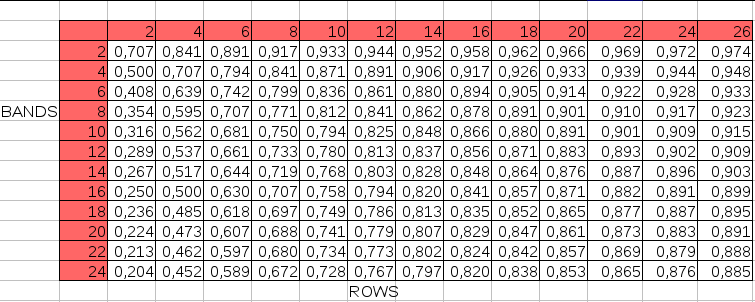
\includegraphics[scale=0.6]{threshold.png}
\centering
\end{figure}

\end{document}
